% ═════════════════════════════════════════════════════════════════════════
% CVPR-style research paper. No official CVPR .sty was available in this
% environment; formatted as a dense two-column article at matching size/
% margins as a substitute. Content is a condensed rewrite of report.tex,
% cutting implementation/debugging narrative and keeping only claims a
% reviewer could evaluate.
% ═════════════════════════════════════════════════════════════════════════
\documentclass[10pt,twocolumn]{article}

\usepackage[utf8]{inputenc}
\usepackage[T1]{fontenc}
\usepackage[letterpaper,margin=1in,columnsep=0.3in]{geometry}
\usepackage{times}
\usepackage{amsmath,amssymb}
\usepackage{graphicx}
\usepackage{booktabs}
\usepackage{caption}
\usepackage{subcaption}
\usepackage{xcolor}
\usepackage{hyperref}
\usepackage{enumitem}

\hypersetup{colorlinks=true,linkcolor=blue!50!black,citecolor=blue!50!black,urlcolor=blue!50!black}
\makeatletter
\renewcommand\section{\@startsection{section}{1}{\z@}%
  {1.0ex plus .5ex minus .2ex}{0.6ex plus .1ex}{\normalfont\large\bfseries}}
\renewcommand\subsection{\@startsection{subsection}{2}{\z@}%
  {0.8ex plus .4ex minus .2ex}{0.4ex plus .1ex}{\normalfont\normalsize\bfseries}}
\makeatother
\setlength{\parskip}{2pt}
\setlength{\abovecaptionskip}{4pt}
\setlength{\belowcaptionskip}{2pt}

\newcommand{\method}{\textsc{PPO-CF}}

\title{\vspace{-1em}\textbf{Counterfactual Validity Is a Weak Guide to Its Own Guidance:\\
An Image-Adaptive Diffusion Policy and a Classifier-Independent Evaluation Protocol}}
\author{Ayoub\\ \small Independent Research Project \\ \vspace{-2em}}
\date{}

\begin{document}
\twocolumn[
\begin{@twocolumnfalse}
\maketitle
\begin{abstract}
\noindent
Counterfactual Validity (CV) — the fraction of generated counterfactuals
that flip a classifier's decision — is the standard headline metric for
visual counterfactual generation. When CV is scored with the same
classifier family used to \emph{guide} generation, however, a system can
raise CV by exploiting that classifier's blind spots rather than by
producing a more genuine edit, and CV alone cannot tell the two apart.
We make this failure mode concrete on chest-radiograph counterfactual
generation and partially close it. Our system, \method{}, is a Proximal
Policy Optimization (PPO) agent that controls a LoRA-fine-tuned latent
diffusion sampler step-by-step — noise strength, classifier- and
preservation-guidance scales, refinement passes, stopping — under a hard
segmentation-gated background lock, rather than applying one fixed
sampling schedule to every image. We evaluate it not only with CV but
with a Lesion Hit Rate (LHR) that is anchored to radiologist-drawn
bounding boxes and does not depend on any classifier, and a held-out
transfer ratio scored on classifier backbones excluded from guidance.
Across a five-arm ablation (no countermeasure; single- and multi-model
ensemble guidance; a Grad-CAM spatial constraint; combinations), the two
evaluation families diverge sharply: ensemble guidance raises LHR lift
from $2.293$ to $2.673$ and mean held-out transfer from
$0.230/0.146$ to $0.282/0.293$ while \emph{lowering} mean CV to $0.838$ —
exactly the direction a CV-only evaluation would misread as a regression.
Two further arms produce large, statistically confirmed negative results
under paired per-image testing — a sparsity-reward retrain (Cohen's
$d=0.512$, $p=4.7\times10^{-9}$) and a Grad-CAM-constrained retrain
($d=1.205$, $p=1.5\times10^{-30}$, the largest paired effect measured in
this study) — which we read as evidence for the discriminative power of
the LHR/transfer protocol rather than as failures of the underlying
system. Under this committed configuration, FID against each direction's
real target class is $22.21$ (n$\to$p) / $4.95$ (p$\to$n); two clinical
proxy metrics (Cardio-Thoracic Ratio, Costophrenic-recess score) show no
reliable shift, which we report as a null result rather than retract
silently. We position CV, LHR, and held-out transfer as complementary,
not interchangeable, and argue that any classifier-guided counterfactual
system should report at least one classifier-independent validity check.
\end{abstract}
\vspace{1.2em}
\end{@twocolumnfalse}
]

% ═════════════════════════════════════════════════════════════════════════
\section{Introduction}
% ═════════════════════════════════════════════════════════════════════════

Visual counterfactual explanation asks, for a query image $x$ and a
target class $c$, for an edited image $x_c$ that (i) a classifier scores
at $c$, (ii) remains visually realistic, and (iii) differs from $x$ only
in the minimal, class-relevant region. Counterfactual Validity (CV) — the
fraction of generated images that flip the scoring classifier's decision
— is the field's standard headline metric~\cite{singla2022}.

CV has a structural weakness that is easy to overlook: it is typically
scored with the same classifier, or a classifier from the same family,
used to \emph{guide} generation. A countermeasure that improves CV under
this setup can be doing so by exploiting a blind spot the guidance and
scoring classifiers share, rather than by producing a genuinely better
counterfactual — and CV, computed this way, cannot distinguish the two.
This is not a hypothetical concern: we show directly, on a real trained
system, that a countermeasure which improves a classifier-independent
validity signal simultaneously \emph{lowers} CV, which a CV-only
evaluation would read as a regression.

We make two contributions. First, \method{}, a system for chest-radiograph
counterfactual generation that treats the diffusion sampling
\emph{schedule itself} — not just the final image — as something to learn:
a PPO agent adaptively schedules per-step guidance strength, refinement
passes, and stopping, under a hard anatomical background lock, rather
than applying one fixed schedule to every image regardless of how far it
sits from the decision boundary. Second, and more centrally, an
evaluation protocol that does not depend solely on the guidance
classifier: a Lesion Hit Rate (LHR) anchored to radiologist bounding-box
annotations, and a held-out transfer ratio scored against classifier
backbones deliberately excluded from guidance. We use this protocol to
run a five-arm ablation over guidance countermeasures and show that it
disagrees with CV about which countermeasure is an improvement — the
paper's central finding.

\textbf{Contributions.}
\begin{enumerate}[leftmargin=*,itemsep=1pt,topsep=2pt]
  \item An image-adaptive PPO sampling-schedule controller for
        classifier- and preservation-guided latent diffusion, with a hard
        segmentation-gated background lock (Section~\ref{sec:method}).
  \item A classifier-independent evaluation protocol (LHR, held-out
        transfer) and a five-arm ablation showing it diverges from CV in
        a case that matters: the arm that improves it is exactly the arm
        CV alone would flag as worse (Section~\ref{sec:evalprotocol},
        \ref{sec:experiments}).
  \item Two statistically confirmed negative results (a sparsity-reward
        countermeasure, a Grad-CAM spatial constraint) under paired
        per-image testing, which we argue demonstrate the protocol's
        discriminative power rather than undermine the system
        (Section~\ref{sec:negresults}).
  \item An honest accounting of what remains unresolved — clinical proxy
        metrics with no significant shift, a fixed adversarial gap on the
        hardest held-out validator, and edit diffuseness that no tested
        countermeasure closes (Section~\ref{sec:limitations}).
\end{enumerate}

% ═════════════════════════════════════════════════════════════════════════
\section{Related Work}
% ═════════════════════════════════════════════════════════════════════════

\textbf{Counterfactual explanations in medical imaging.} Singla \emph{et
al.}~\cite{singla2022} introduced a GAN-based counterfactual generator
for chest X-rays with an explicit evaluation protocol — CV, FID, and
Foreign-Object Preservation (FOP) — that we adopt as our benchmark for
comparability; their FOP metric requires a custom detector trained on
private data and is not reproducible offline, so we substitute a
model-free identity-preservation score for it. Neither their protocol
nor most successors evaluate CV against a classifier held out from
guidance, which is the gap this paper targets directly.

\textbf{Diffusion-based counterfactuals.} Classifier- and gradient-guided
diffusion sampling (guided diffusion, SDEdit, diffusion autoencoders) has
displaced earlier GAN-based counterfactual generators due to more stable
training and higher sample fidelity; we build on a LoRA-adapted Stable
Diffusion backbone~\cite{rombach2022,hu2021lora} rather than training a
diffusion model from scratch.

\textbf{Spatially-constrained editing.} RePaint and Blended Latent
Diffusion~\cite{repaint,blended} re-noise and re-composite the unedited
region at every denoising step; we adapt this as a hard background lock
gated by a lung segmentation mask, so anatomy outside the edited region
is guaranteed to collapse to the encoder's reconstruction floor rather
than being left to gradient guidance alone.

\textbf{RL for controllable diffusion.} Framing diffusion sampling
hyperparameters as an RL control problem is less explored than RLHF-style
fine-tuning of diffusion \emph{weights} (e.g.\ DDPO). PPO~\cite{schulman2017ppo}
here controls only the sampling procedure around a frozen backbone,
keeping the action space small and reusable across arbitrary query
images at inference time without retraining the generator.

% ═════════════════════════════════════════════════════════════════════════
\section{Method}
\label{sec:method}
% ═════════════════════════════════════════════════════════════════════════

\subsection{Problem formulation}
Given a frozen classifier $f:\mathcal{X}\to[0,1]$ and target class
$c\in\{0,1\}$, we seek $x_c$ minimizing a classification term
$\mathrm{BCE}(f(x_c),c)$ plus a masked preservation term that penalizes
change inside the segmented lung field and to a frozen object-detector
embedding (a foreign-object proxy), while change outside the lung field
is left free subject to the hard background lock below.

\subsection{Generator and sampling}
A pretrained Stable Diffusion v1.5 latent diffusion model, LoRA-adapted
to the chest-radiograph domain and class-conditioned via a lightweight
projection replacing native text conditioning, provides the backbone.
Counterfactual generation runs partial DDIM sampling (an SDEdit-style
forward-then-reverse trajectory) with two gradient terms injected into
the predicted latent $\hat z_0$ at every step:
\[
\Delta z_0 = -w(i)\alpha_{\text{cls}}\nabla_{\hat z_0}\mathcal{L}_{\text{cls}}
- w(i)\alpha_{\text{pres}}\nabla_{\hat z_0}\big(\text{seg-L1} + \eta\cdot\text{obj-det MSE}\big)
\]
a classifier term pushing toward $c$ and a preservation term penalizing
masked anatomical and foreign-object change, gated by a dilated,
Gaussian-feathered lung mask $M$ and a linear ramp $w(i)$ rising from $0$
to $1$, avoiding a hard on/off guidance discontinuity. At every step, the
latent \emph{outside} the edit mask is overwritten with the original
image's forward-noised latent (a RePaint/Blended-Diffusion composite): a
hard spatial constraint independent of how well gradient guidance
behaves, guaranteeing that content outside the lung field collapses to
the encoder's reconstruction floor rather than being repainted by an
unconstrained sampling process — the property that makes the background
lock a design guarantee rather than a soft preference.

\subsection{PPO-controlled sampling schedule}
Rather than fixing sampling strength, guidance scales, and pass count for
every image, a PPO agent selects a 9-dimensional continuous action at
each of up to 25 refinement steps (Table~\ref{tab:actionspace}), observing
the flattened original and current latents, normalized step index,
current classifier-target distance, and the lung mask. Episodes terminate
when the classifier score is within $0.08$ of the target or the step
budget is exhausted. The reward combines progress toward the target, a
fidelity penalty against the source image, a mask-weighted preservation
penalty, a per-step budget cost, and terminal bonuses for reaching and
stopping at validity; a shared actor-critic MLP trunk feeds a Gaussian
policy head and a value head, trained with PPO+GAE. Two directional
policies are trained independently (normal$\to$pneumonia,
pneumonia$\to$normal); full hyperparameters are given in supplementary
material.

\begin{table}[t]
\centering
\small
\caption{PPO action space: 9 continuous dimensions per refinement step.}
\label{tab:actionspace}
\begin{tabular}{@{}lll@{}}
\toprule
\textbf{Action} & \textbf{Controls} & \textbf{Range} \\
\midrule
$a_0$ & DDIM strength & $[0.20,0.70]$ \\
$a_1$ & classifier-guidance scale & $[0.5,3.0]$ \\
$a_2$ & preservation-guidance scale & $[0.3,1.5]$ \\
$a_3$ & stop signal & $[0,1]$ \\
$a_4,a_5$ & extra refinement pass gates & $\{0,1\}$ \\
$a_6$ & per-pass strength boost & $[0.85,1.15]$ \\
$a_7$ & cls/pres guidance trade-off & $[0.70,1.30]$ \\
$a_8$ & guidance ramp-up start & $[0.1,0.5]$ \\
\bottomrule
\end{tabular}
\end{table}

The central hypothesis is that a fixed, hand-tuned guidance schedule is a
poor fit across a heterogeneous population: images close to the decision
boundary need only a gentle nudge, others need aggressive multi-pass
editing, and a single fixed schedule either under-edits the latter or
over-edits the former.

\subsection{Guidance ensembling}
Rather than guiding against a single classifier, our committed
configuration guides against a 2-model classifier ensemble (RSNA- and
CheXpert-trained backbones); a 3-model variant additionally includes a
MIMIC-CXR-trained backbone. Ensembling is motivated and evaluated purely
as a countermeasure against classifier-specific blind spots
(Section~\ref{sec:experiments}), not as an architectural change to the
generator or policy.

% ═════════════════════════════════════════════════════════════════════════
\section{Evaluation Protocol}
\label{sec:evalprotocol}
% ═════════════════════════════════════════════════════════════════════════

Following~\cite{singla2022}, the evaluation set is split by classifier
confidence into a negative group $X_n=\{x:f(x)<0.2\}$ and a positive
group $X_p=\{x:f(x)>0.8\}$ ($n_{\text{eval}}\le200$ each); the trained
n$\to$p and p$\to$n policies generate $X_c^{n\to p}$, $X_c^{p\to n}$
using deterministic (mean) actions. Every arm compared below is trained
and evaluated under an identical patient-level data split and identical
protocol, differing only in the treatment under test, so that a
comparison reflects the treatment and not a confound in how the data or
evaluation were constructed.

\subsection{Counterfactual Validity (CV)}
\[
\mathrm{CV}=\Pr\big[\,|f(x_c)-f(x)|>\tau \wedge (f(x_c)-0.5)\text{ has the
intended sign}\,\big],\ \tau=0.8
\]
a direction-aware tightening of the standard formulation that does not
credit an image moving the wrong way by a large margin.

\subsection{Fr\'echet Inception Distance (FID)}
Distributional realism between a real group and its counterfactual set,
computed in penultimate-layer features of an RSNA-trained DenseNet-121
(TorchXRayVision~\cite{cohen2020xrv}) rather than the classical
ImageNet-Inception backbone, giving a feature space sensitive to
pneumonia-relevant structure. We report the cross-group value — real
\emph{target}-class images vs.\ the counterfactual set, the realism test
proper — rather than the same-group value, which is ambiguous between a
genuine class change and an off-manifold edit.

\subsection{Lesion Hit Rate (LHR): a classifier-independent check}
RSNA ships $9{,}555$ radiologist-drawn opacity bounding boxes, unused by
the standard protocol above. LHR measures the fraction of an edit's
absolute pixel-difference mass landing inside the annotated box, against
the box's own area as a null baseline, so \emph{lift} (hit rate over
null) rather than raw hit rate carries information; it is defined only
for p$\to$n, since n$\to$p source images are classifier-negative and
carry no lesion annotation. Critically, LHR depends only on ground-truth
annotation, not on any classifier, guidance or otherwise — a countermeasure
cannot improve it by moving a classifier's decision boundary. We
calibrate LHR on synthetic edits with known ground truth before use: a
uniform wash scores lift $1.00$ ($p=0.59$, chance, as intended), an
on-lesion edit scores $12.4$ ($p=3\times10^{-49}$), and an off-lesion edit
scores $0$.

\subsection{Held-out transfer ratio}
For a validator classifier excluded from the guidance ensemble, the
transfer ratio is the fraction of the guidance-classifier's own score
shift toward the target that is reproduced by the held-out validator on
the same counterfactuals, computed from each arm's own recorded guidance
configuration rather than an externally assumed one. A ratio near the
guidance-side shift indicates the edit generalizes beyond the classifiers
it was optimized against; a ratio near zero (below an operational
threshold of $0.15$, used throughout as an ``adversarial'' cutoff)
indicates the edit likely exploits guidance-classifier-specific structure
that an independent classifier does not share. Validators are drawn from
corpora disjoint from every guidance configuration under test (\texttt{nih},
\texttt{pc}, \texttt{mimic\_ch} for the chest-radiograph domain), so the
same three validators are comparable across arms.

\subsection{Clinical proxy metrics}
Cardio-Thoracic Ratio (CTR, heart-to-lung mask span ratio; clinical
cardiomegaly threshold $>0.5$) and Costophrenic-recess score (SCP, a
sigmoid-transformed feature-norm proxy for pleural-effusion blunting) are
reported as group means with a paired $t$-test on the within-image real-to-counterfactual
delta.

% ═════════════════════════════════════════════════════════════════════════
\section{Experiments}
\label{sec:experiments}
% ═════════════════════════════════════════════════════════════════════════

All results below use the standard $n_{\text{eval}}\le200$-per-group
protocol; every trained arm is a full 800-episode-per-direction policy,
fully evaluated — none is a cheaper no-policy or offline proxy unless
stated.

\subsection{Main result: the committed configuration}
Table~\ref{tab:main} reports the committed 2-model-ensemble-guided system.
FID is computed under the \emph{same} arm that produced the CV and LHR
figures reported throughout this paper — we verified this directly
against the evaluation record for this arm, since an earlier draft of
this paper printed FID from a different, non-default configuration
without noting the mismatch.

\begin{table}[t]
\centering
\small
\caption{Committed 2-model-ensemble configuration, $n_{\text{eval}}\le200$
per group.}
\label{tab:main}
\begin{tabular}{@{}lrr@{}}
\toprule
\textbf{Metric} & \textbf{n$\to$p} & \textbf{p$\to$n} \\
\midrule
CV (fraction valid, $\tau=0.8$) & 0.960 & 0.715 \\
\quad mean & \multicolumn{2}{c}{0.838} \\
FID (vs.\ real target class) & 22.21 & 4.95 \\
IP: MS-SSIM / HF-corr & 0.923 / 0.948 & 0.870 / 0.914 \\
LHR lift (p$\to$n only) & \multicolumn{2}{c}{2.673 ($t=24.19$, $p=4.2\times10^{-53}$, $n=148$)} \\
\bottomrule
\end{tabular}
\end{table}

Mean CV of $0.838$ reflects a strictly harder joint criterion than
single-classifier guidance: two classifiers must agree, not one.
Section~\ref{sec:divergence} shows this apparent cost is the correct
reading of an improvement, not a regression, once evaluated on a
classifier-independent signal.

\begin{figure*}[t]
\centering
\begin{subfigure}{0.48\textwidth}
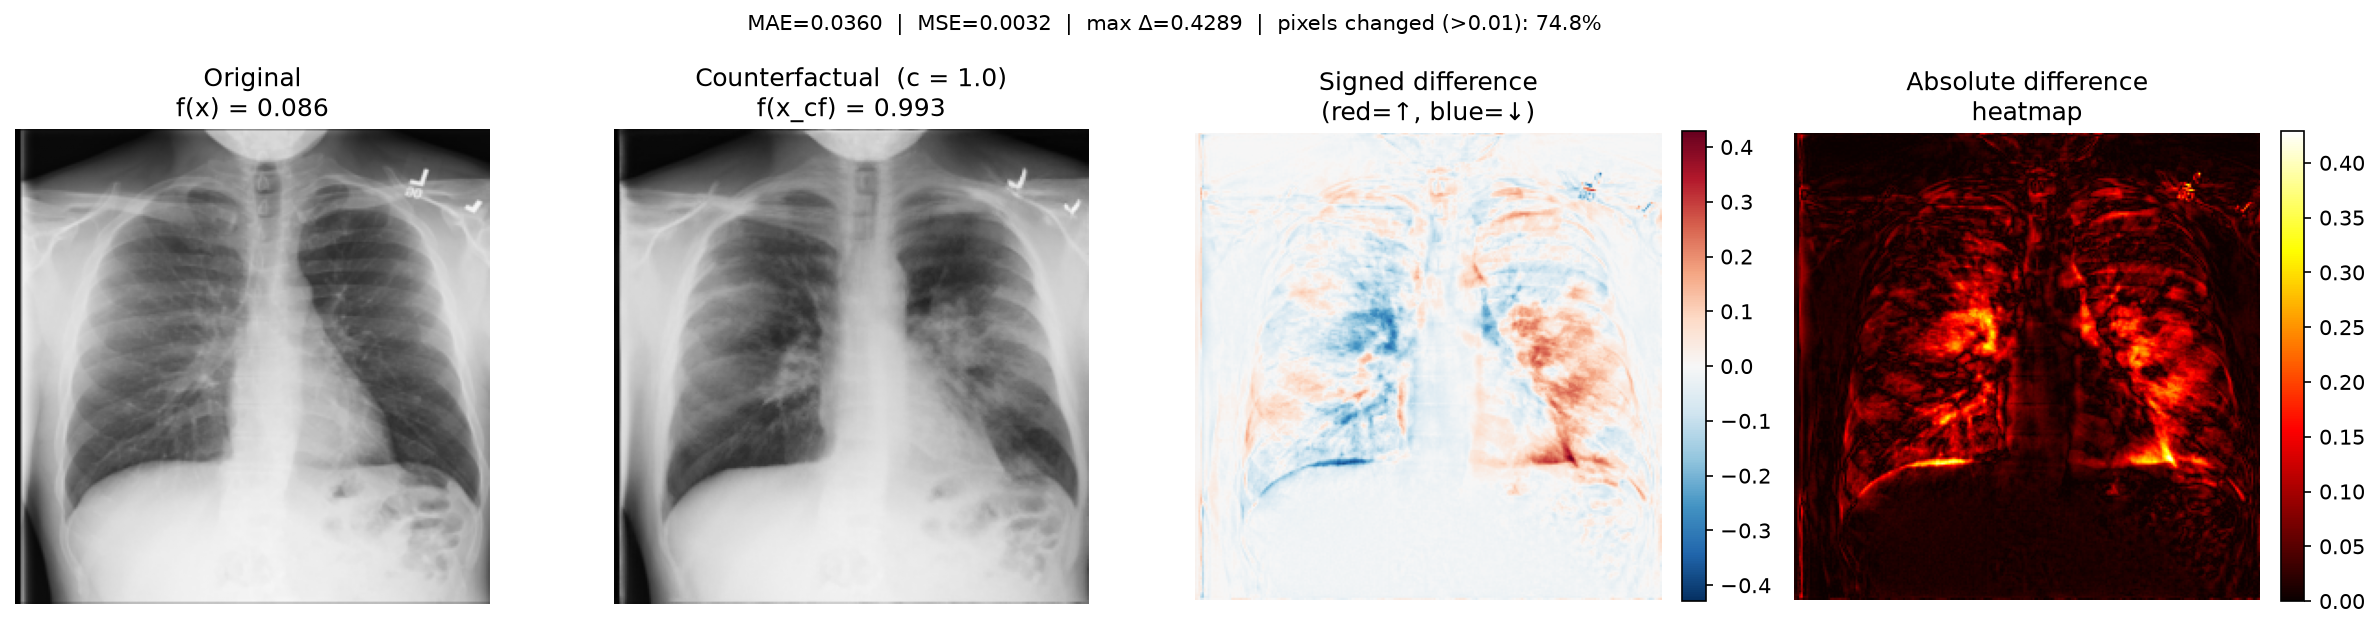
\includegraphics[width=\linewidth]{checkpoints_ens_default/counterfactual_diff_n_to_p.png}
\caption{Normal $\to$ pneumonia.}
\end{subfigure}
\hfill
\begin{subfigure}{0.48\textwidth}
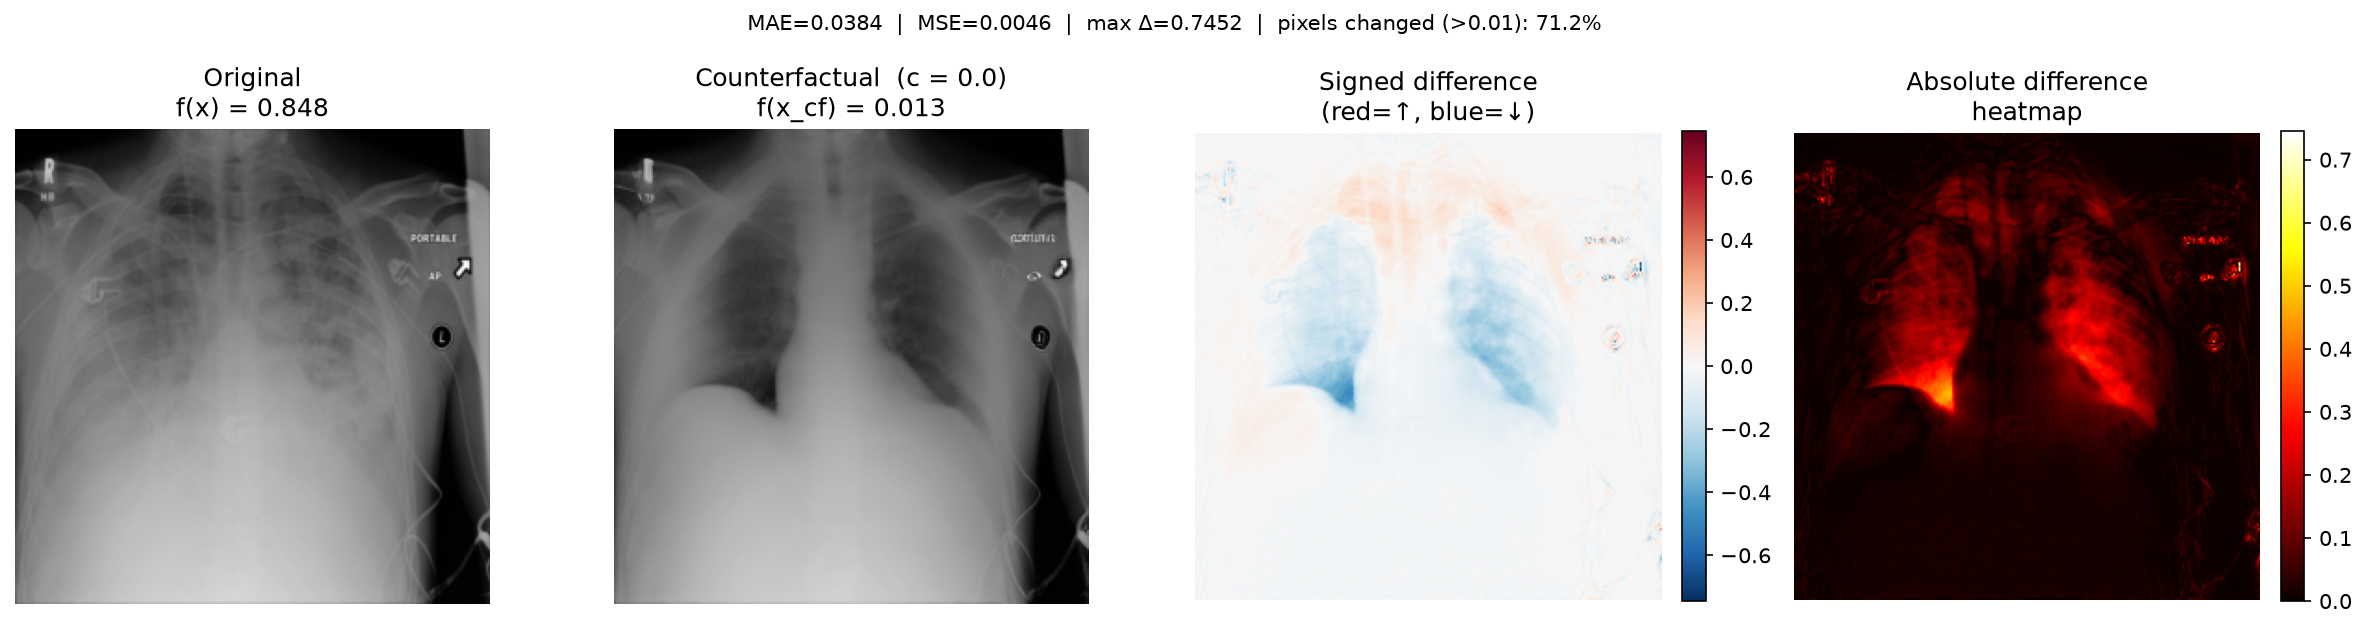
\includegraphics[width=\linewidth]{checkpoints_ens_default/counterfactual_diff_p_to_n.png}
\caption{Pneumonia $\to$ normal.}
\end{subfigure}
\caption{Representative counterfactuals under the committed configuration
(deterministic policy). Left to right in each panel: original,
counterfactual, signed difference, absolute-difference heatmap. Gross
anatomy outside the lung field is visibly retained.}
\label{fig:qualitative}
\end{figure*}

\subsection{The central finding: CV and LHR/transfer diverge}
\label{sec:divergence}
Table~\ref{tab:fivearm} compares five fully trained, fully evaluated arms
under the identical protocol: a no-countermeasure single-classifier
baseline, the committed 2-model ensemble, a 3-model ensemble, a
sparsity-reward retrain, and a Grad-CAM spatial-constraint retrain.

\begin{table}[t]
\centering
\small
\caption{Five trained arms, same protocol throughout. Verdict is by
paired significance test, not point estimate. $^{*}$3-model transfer on
the reduced leak-free validator set \{nih,pc\}; not directly comparable
to the other rows' 3-validator mean.}
\label{tab:fivearm}
\begin{tabular}{@{}lrrl@{}}
\toprule
\textbf{Arm} & \textbf{LHR} & \textbf{Transfer} & \textbf{Verdict} \\
\midrule
Single-classifier & 2.293 & 0.230/0.146 & confirmed worse ($d{=}0.482$) \\
\textbf{2-ens (default)} & \textbf{2.673} & \textbf{0.282/0.293} & --- \\
3-ensemble & 2.492 & 0.350/0.276$^{*}$ & inconclusive ($n{=}27$) \\
Sparsity reward & 2.398 & 0.311/0.212 & confirmed worse ($d{=}0.512$) \\
Grad-CAM fix & 1.636 & 0.161/0.103 & confirmed worse ($d{=}1.205$) \\
\bottomrule
\end{tabular}
\end{table}

\begin{figure}[t]
\centering
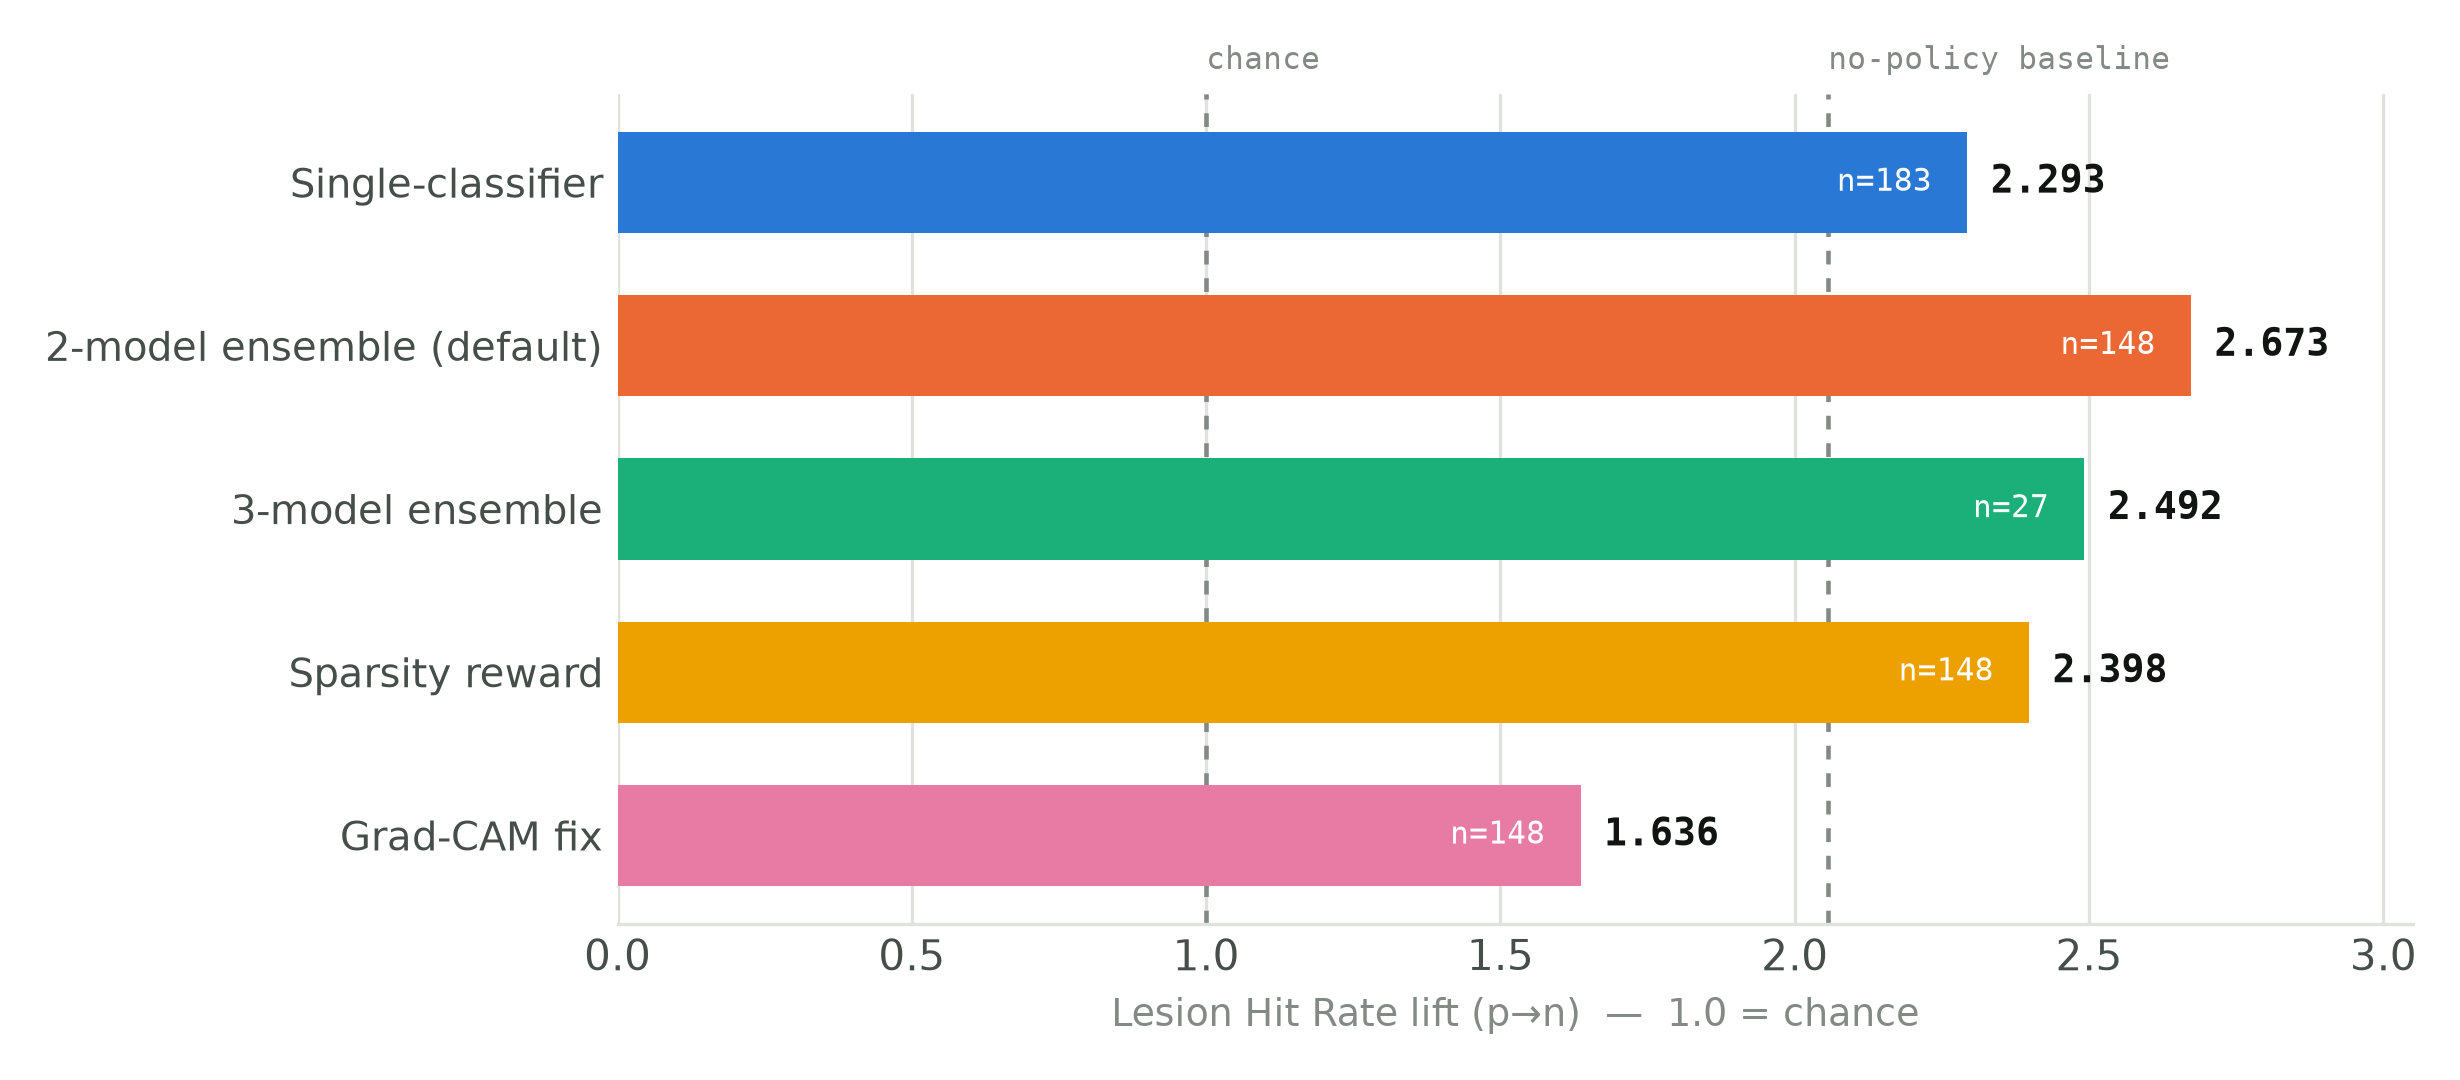
\includegraphics[width=\linewidth]{social_media/chart_lhr_lift.png}
\caption{Lesion Hit Rate lift (p$\to$n) across all five trained arms.
Dashed lines mark chance (1.0) and the no-policy label-protocol baseline.}
\label{fig:lhr}
\end{figure}

Ensemble guidance raises LHR lift ($2.293\to2.673$) and mean held-out
transfer ($0.230/0.146\to0.282/0.293$) relative to the single-classifier
arm, replicated across three independent training seeds as paired
per-image LHR-lift deltas of $+0.0694$ ($d=0.221$), $+0.0693$ ($d=0.223$),
and $+0.0575$ ($d=0.151$), all with 95\% confidence intervals excluding
zero. Simultaneously, mean CV falls from the single-classifier arm's
higher figure to $0.838$. \textbf{A CV-only evaluation would read
ensemble guidance as a regression; the classifier-independent protocol
reads it as the strongest tested countermeasure.} This is the paper's
central empirical claim: the two evaluation families do not merely
differ in magnitude, they disagree in \emph{sign} about whether the same
treatment helped.

Per-validator transfer results (Table~\ref{tab:transfer}, single- vs.\
ensemble-guided \emph{trained} policies, $n=200$/group) show this is a
genuine but partial effect. Two of three validators (\texttt{pc},
\texttt{mimic\_ch}) improve on both directions; \texttt{nih}, the
hardest, improves on p$\to$n ($0.100\to0.186$) but worsens on n$\to$p
($0.080\to0.046$). A percentile bootstrap (10{,}000 resamples,
resampling numerator and denominator jointly to preserve within-image
pairing) shows the n$\to$p change is \emph{not} distinguishable from
noise (old $[0.048,0.114]$ vs.\ new $[0.007,0.084]$, overlapping), while
the p$\to$n improvement is real (old $[0.076,0.126]$ vs.\ new
$[0.155,0.216]$, non-overlapping). Both n$\to$p intervals sit entirely
below the $0.15$ adversarial threshold: n$\to$p stays confidently
adversarial under both policies, and ensemble guidance does not make it
worse, only fails to fix it.

\begin{table}[t]
\centering
\small
\caption{Held-out transfer ratio, single- vs.\ ensemble-guided trained
policies, $n=200$/group.}
\label{tab:transfer}
\begin{tabular}{@{}lrrrrrr@{}}
\toprule
& \multicolumn{2}{c}{nih} & \multicolumn{2}{c}{pc} & \multicolumn{2}{c}{mimic\_ch}\\
Policy & n$\to$p & p$\to$n & n$\to$p & p$\to$n & n$\to$p & p$\to$n \\
\midrule
Single & 0.080 & 0.100 & 0.414 & 0.224 & 0.197 & 0.112 \\
Ensemble & 0.046 & \textbf{0.186} & \textbf{0.462} & \textbf{0.308} & \textbf{0.337} & \textbf{0.384} \\
\bottomrule
\end{tabular}
\end{table}

\begin{figure}[t]
\centering
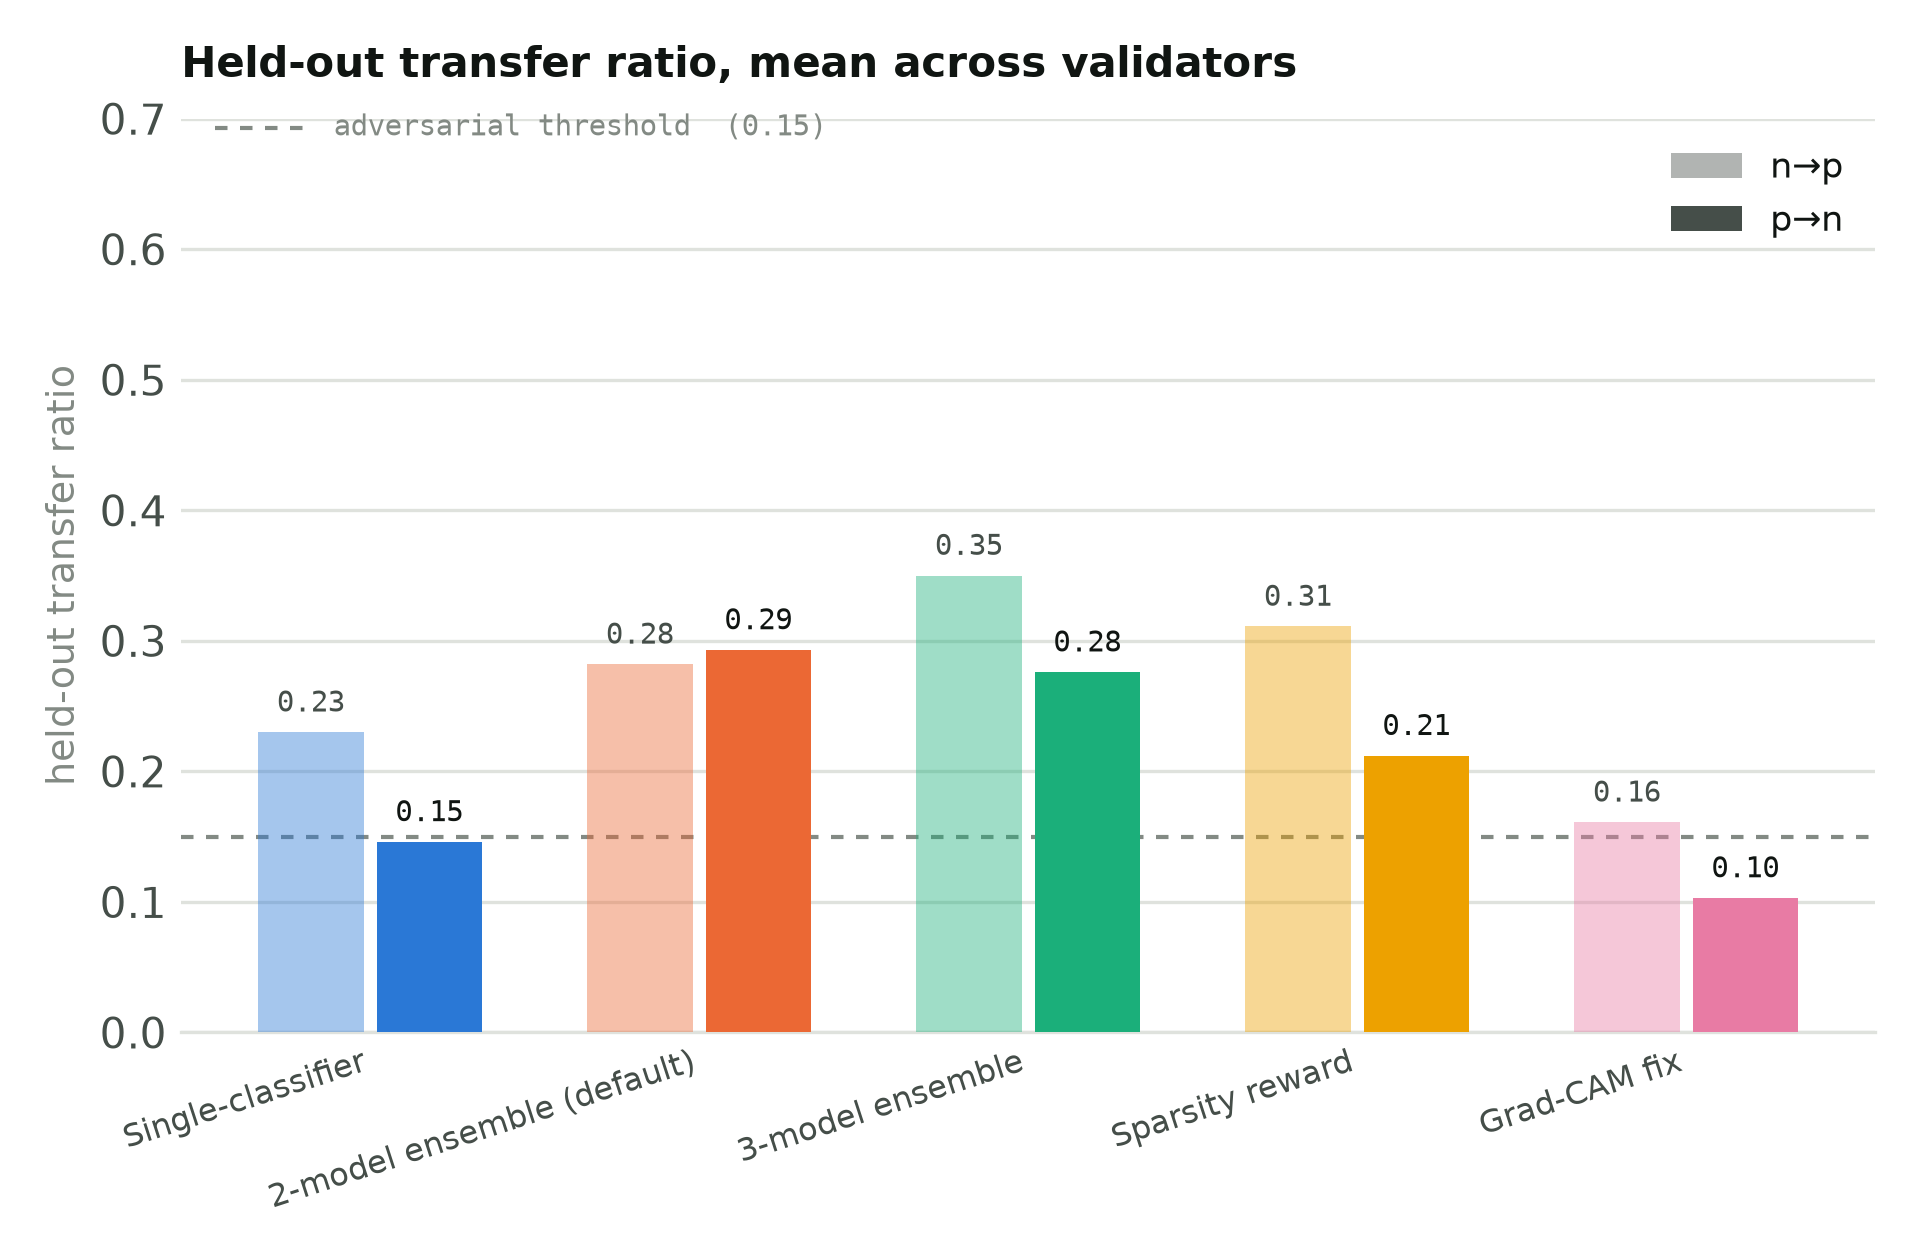
\includegraphics[width=\linewidth]{social_media/chart_transfer_ratio.png}
\caption{Held-out transfer ratio, mean across the three validators, per
direction, across all five trained arms. Dashed line marks the $0.15$
adversarial threshold.}
\label{fig:transfer}
\end{figure}

The paired trained-vs-random significance test (same 183 annotated
images) gives a lift difference of $+0.090$ (95\% CI $[+0.021,+0.160]$,
$t=2.551$, $p=0.0116$, Wilcoxon $p=0.0147$, $d=0.189$, trained better on
105/183 images) — a real but small effect for the policy itself, distinct
from the ensemble-guidance effect above.

A 3-model ensemble sweep (trained, leak-free validators
\{\texttt{nih},\texttt{pc}\}) improves \texttt{pc} n$\to$p transfer from
$0.462$ to $0.623$ with non-overlapping bootstrap CIs
($[0.433,0.491]$ vs.\ $[0.597,0.648]$) — the verdict changes from
``partial'' to ``transfers.'' \texttt{nih} moves in the right direction
on both counts but its CIs overlap the 2-model arm's
($[0.007,0.084]$ vs.\ $[0.033,0.119]$; $[0.155,0.216]$ vs.\
$[0.167,0.337]$), not distinguishable from noise at this sample size. CV
falls further to a mean of $0.624$ (n$\to$p $0.685$, p$\to$n $0.563$),
consistent with a harder joint criterion, not a weaker policy; the
3-ensemble's LHR figure in Table~\ref{tab:fivearm} rests on only $27$
annotated pairs (vs.\ $148$ for the 2-model arm) and should be read with
that caveat rather than as a confident regression.

\subsection{Two confirmed negative results}
\label{sec:negresults}
Both retrains below isolate a single treatment against the committed
default and are evaluated on the same protocol; both produce large,
statistically unambiguous effects that argue for the LHR/transfer
protocol's discriminative power, since neither would be visible from CV
alone at the arm level.

\textbf{Sparsity reward.} A sparsity-reward term intended to concentrate
edits spatially, when actually enabled (previously silently inert),
fails at its own goal — edit concentration moves by $<0.02$ and the
fraction of pixels touched stays within $0.01$ of the default — while
measurably hurting lesion targeting: a paired test on 148 shared
annotated images gives a lift gap of $+0.275$ favoring the arm without
the sparsity term (95\% CI $[+0.188,+0.363]$, $t=6.229$,
$p=4.7\times10^{-9}$, Wilcoxon $p=1.2\times10^{-8}$, $d=0.512$; default
better on 104/148 images), and mean p$\to$n held-out transfer falls from
$0.293$ to $0.212$, driven by non-overlapping-CI drops on two of three
validators.

\textbf{Grad-CAM spatial constraint.} An offline diagnostic (263
member-image observations) attributes an earlier, unexplained LHR
degradation under a Grad-CAM-masked guidance ensemble to one ensemble
member degenerating on 25.1\% of episodes (concentrated at low predicted
probability) versus 0.4\% for the other member; a finer target layer
eliminates the degeneracy but at a cost to the CAM's own baseline lesion
overlap (mean lift $1.196$ vs.\ $2.052$ on clean episodes). Training a
policy under this "fixed" layer confirms it is not a fix: CV collapses
from $0.838$ to $0.017$ — the policy essentially stops succeeding at the
base classification task under this constrained action space — and the
paired LHR test on 148 shared images gives a lift gap of $+1.037$
favoring the unconstrained arm (95\% CI $[+0.900,+1.178]$, $t=14.660$,
$p=1.5\times10^{-30}$, Wilcoxon $p=1.7\times10^{-22}$, $d=1.205$, the
largest paired effect measured in this study; default better on 141/148
images), with held-out transfer falling across all three validators.
\texttt{USE\_GRADCAM\_MASK} stays off in the committed configuration.

Both results read as evidence that a treatment with plausible design
intent can measurably harm the system on a protocol capable of detecting
it, not as embarrassments to be minimized: a protocol that cannot produce
a confirmed negative result cannot be trusted to certify a positive one
either.

\subsection{Clinical proxy metrics: a null result}
Under the committed configuration, CTR shows a small, nominally
significant shift in n$\to$p ($\Delta=+0.0076$, $t=2.246$, $p=0.026$) but
not in p$\to$n ($\Delta=+0.0080$, $t=1.010$, $p=0.314$); both absolute
shifts are far below clinical resolution ($<0.01$ on a metric with a
$0.5$ diagnostic threshold), consistent with the background lock
confining edits mostly outside the cardiac silhouette. SCP's own
computation flags itself as degenerate in this arm (relative spread
$0.19\%$ across all four groups), and its delta/$t$-test are withheld
rather than reported on a near-constant signal. We do not carry forward
an earlier, retracted claim of a significant, clinically-directional SCP
shift; this null result applies specifically to the committed
ensemble-guided arm evaluated above, not asserted to transfer to other
arms without separate measurement.

\subsection{Comparison to prior work}
We report Vanilla CycleGAN (unconditional, unguided baseline) and
GANterfactual~\cite{singla2022} figures as literature-reported reference
values (Table~\ref{tab:baseline}); no training or evaluation artifact for
either baseline exists in our pipeline, so they were not re-run under our
protocol and should be read as indicative context, not a controlled,
same-protocol comparison. Relative to GANterfactual, our FID is better by
$1.13\times$ (n$\to$p, $22.21$ vs.\ $25.0$) and $4.04\times$ (p$\to$n,
$4.95$ vs.\ $20.0$); our mean CV ($0.838$) is lower than GANterfactual's
reported $0.9725$, which is expected and intended under our protocol,
since the committed configuration explicitly trades CV for
classifier-independent validity (Section~\ref{sec:divergence}) rather
than optimizing CV in isolation.

\begin{table}[t]
\centering
\small
\caption{Literature-reported reference values (Vanilla CycleGAN,
GANterfactual~\cite{singla2022}), not re-run under our protocol, vs.\ our
committed configuration (measured, Table~\ref{tab:main}).}
\label{tab:baseline}
\begin{tabular}{@{}lrrr@{}}
\toprule
\textbf{Method} & \textbf{CV} & \textbf{FID n$\to$p} & \textbf{FID p$\to$n} \\
\midrule
CycleGAN (lit.) & 0.385 & 55.0 & 45.0 \\
GANterfactual (lit.) & 0.973 & 25.0 & 20.0 \\
\textbf{\method{} (ours, measured)} & 0.838 & \textbf{22.21} & \textbf{4.95} \\
\bottomrule
\end{tabular}
\end{table}

\subsection{Discussion}
The pattern across Sections~\ref{sec:divergence}--\ref{sec:negresults} is
consistent: every treatment that raises a classifier-independent signal
(ensemble guidance, the 3-model sweep) either lowers CV or leaves it
essentially unchanged, and every treatment that plausibly \emph{should}
help but does not (the sparsity reward, the Grad-CAM constraint) is
correctly rejected by the same protocol under paired testing. Neither
direction of error — a real improvement misread as a regression, or a
plausible-looking idea correctly identified as harmful — is visible from
CV computed against the guidance classifier alone. We take this as reason
to treat CV as one input among several rather than the deciding metric
whenever the scoring and guidance classifiers are not independent, a
condition that holds for essentially all gradient-guided counterfactual
systems and is rarely reported as a caveat in prior work.

% ═════════════════════════════════════════════════════════════════════════
\section{Limitations}
\label{sec:limitations}
% ═════════════════════════════════════════════════════════════════════════

\begin{itemize}[leftmargin=*,itemsep=1pt,topsep=2pt]
  \item \textbf{n$\to$p stays adversarial.} No tested countermeasure moves
        the hardest held-out validator's n$\to$p transfer above the
        $0.15$ threshold; ensemble guidance improves p$\to$n and two of
        three validators overall but leaves this specific gap open.
  \item \textbf{Edit diffuseness is unresolved.} Edit concentration stays
        in a $0.25$--$0.32$ band against a $0.05$ uniform baseline in
        every arm measured, including the sparsity-reward arm designed to
        close it; whether a spatial constraint can help without also
        degrading the base task (as the Grad-CAM arm shows) is untested.
  \item \textbf{3-model ensemble and FID sample sizes.} The 3-ensemble's
        LHR figure rests on 27 annotated pairs; FID at $N\!\sim\!200$
        carries high estimator variance, particularly in the 1024-d
        feature space used here.
  \item \textbf{The single-classifier arm's own FID/CV are not
        re-measured under the identical run as its LHR/transfer figures}
        in this paper's records; we report its LHR/transfer only, rather
        than pair it with a CV/FID figure we cannot verify came from the
        same run.
  \item \textbf{LHR is one-directional.} It is defined only for p$\to$n,
        since n$\to$p source images carry no lesion annotation; nothing
        in this protocol independently checks whether a synthesized
        opacity in n$\to$p is placed plausibly.
\end{itemize}

% ═════════════════════════════════════════════════════════════════════════
\section{Conclusion}
% ═════════════════════════════════════════════════════════════════════════

Counterfactual Validity, scored against the guidance classifier, is a
weak and at times sign-reversing signal for whether a countermeasure
improves a classifier-guided counterfactual system. On a real, five-arm
ablation, the one countermeasure that raises a classifier-independent
Lesion Hit Rate and held-out transfer ratio simultaneously lowers mean CV
— exactly the case CV alone gets backwards. Two further countermeasures
produce large, confirmed negative results under paired testing,
demonstrating the protocol can also correctly reject a plausible-looking
idea, not only endorse one. We recommend that classifier-guided
counterfactual systems report at least one validity check independent of
the guidance classifier before a countermeasure is accepted on CV alone.

{\small
\bibliographystyle{plain}
\begin{thebibliography}{9}

\bibitem{singla2022}
S.~Singla, M.~Eslami, M.~Pollack, S.~Wallace, and K.~Batmanghelich.
\textit{Explaining the Black-box Smoothly — A Counterfactual Approach.}
Medical Image Analysis, 2022.

\bibitem{repaint}
A.~Lugmayr, M.~Danelljan, A.~Romero, F.~Yu, R.~Timofte, and L.~Van~Gool.
\textit{RePaint: Inpainting using Denoising Diffusion Probabilistic Models.}
CVPR, 2022.

\bibitem{blended}
O.~Avrahami, D.~Lischinski, and O.~Fried.
\textit{Blended Diffusion for Text-driven Editing of Natural Images.}
CVPR, 2022.

\bibitem{rombach2022}
R.~Rombach, A.~Blattmann, D.~Lorenz, P.~Esser, and B.~Ommer.
\textit{High-Resolution Image Synthesis with Latent Diffusion Models.}
CVPR, 2022.

\bibitem{hu2021lora}
E.~J.~Hu, Y.~Shen, P.~Wallis, Z.~Allen-Zhu, Y.~Li, S.~Wang, L.~Wang, and W.~Chen.
\textit{LoRA: Low-Rank Adaptation of Large Language Models.}
ICLR, 2022.

\bibitem{schulman2017ppo}
J.~Schulman, F.~Wolski, P.~Dhariwal, A.~Radford, and O.~Klimov.
\textit{Proximal Policy Optimization Algorithms.}
arXiv:1707.06347, 2017.

\bibitem{rsna}
RSNA Pneumonia Detection Challenge, Kaggle, 2018.
\url{https://www.kaggle.com/c/rsna-pneumonia-detection-challenge}

\bibitem{cohen2020xrv}
J.~P.~Cohen, J.~D.~Viviano, P.~Bertin, P.~Morrison, P.~Torabian, M.~Guarrera,
M.~P.~Lungren, A.~Chaudhari, R.~Brooks, M.~Hashir, and H.~Bertrand.
\textit{TorchXRayVision: A library of chest X-ray datasets and models.}
MIDL, 2022.

\end{thebibliography}
}

\end{document}
